\section{Run-time View}
These sequence diagrams shows how the different components interact through each other when the main features are used by various actors.

\begin{figure}[H]
    \centering
    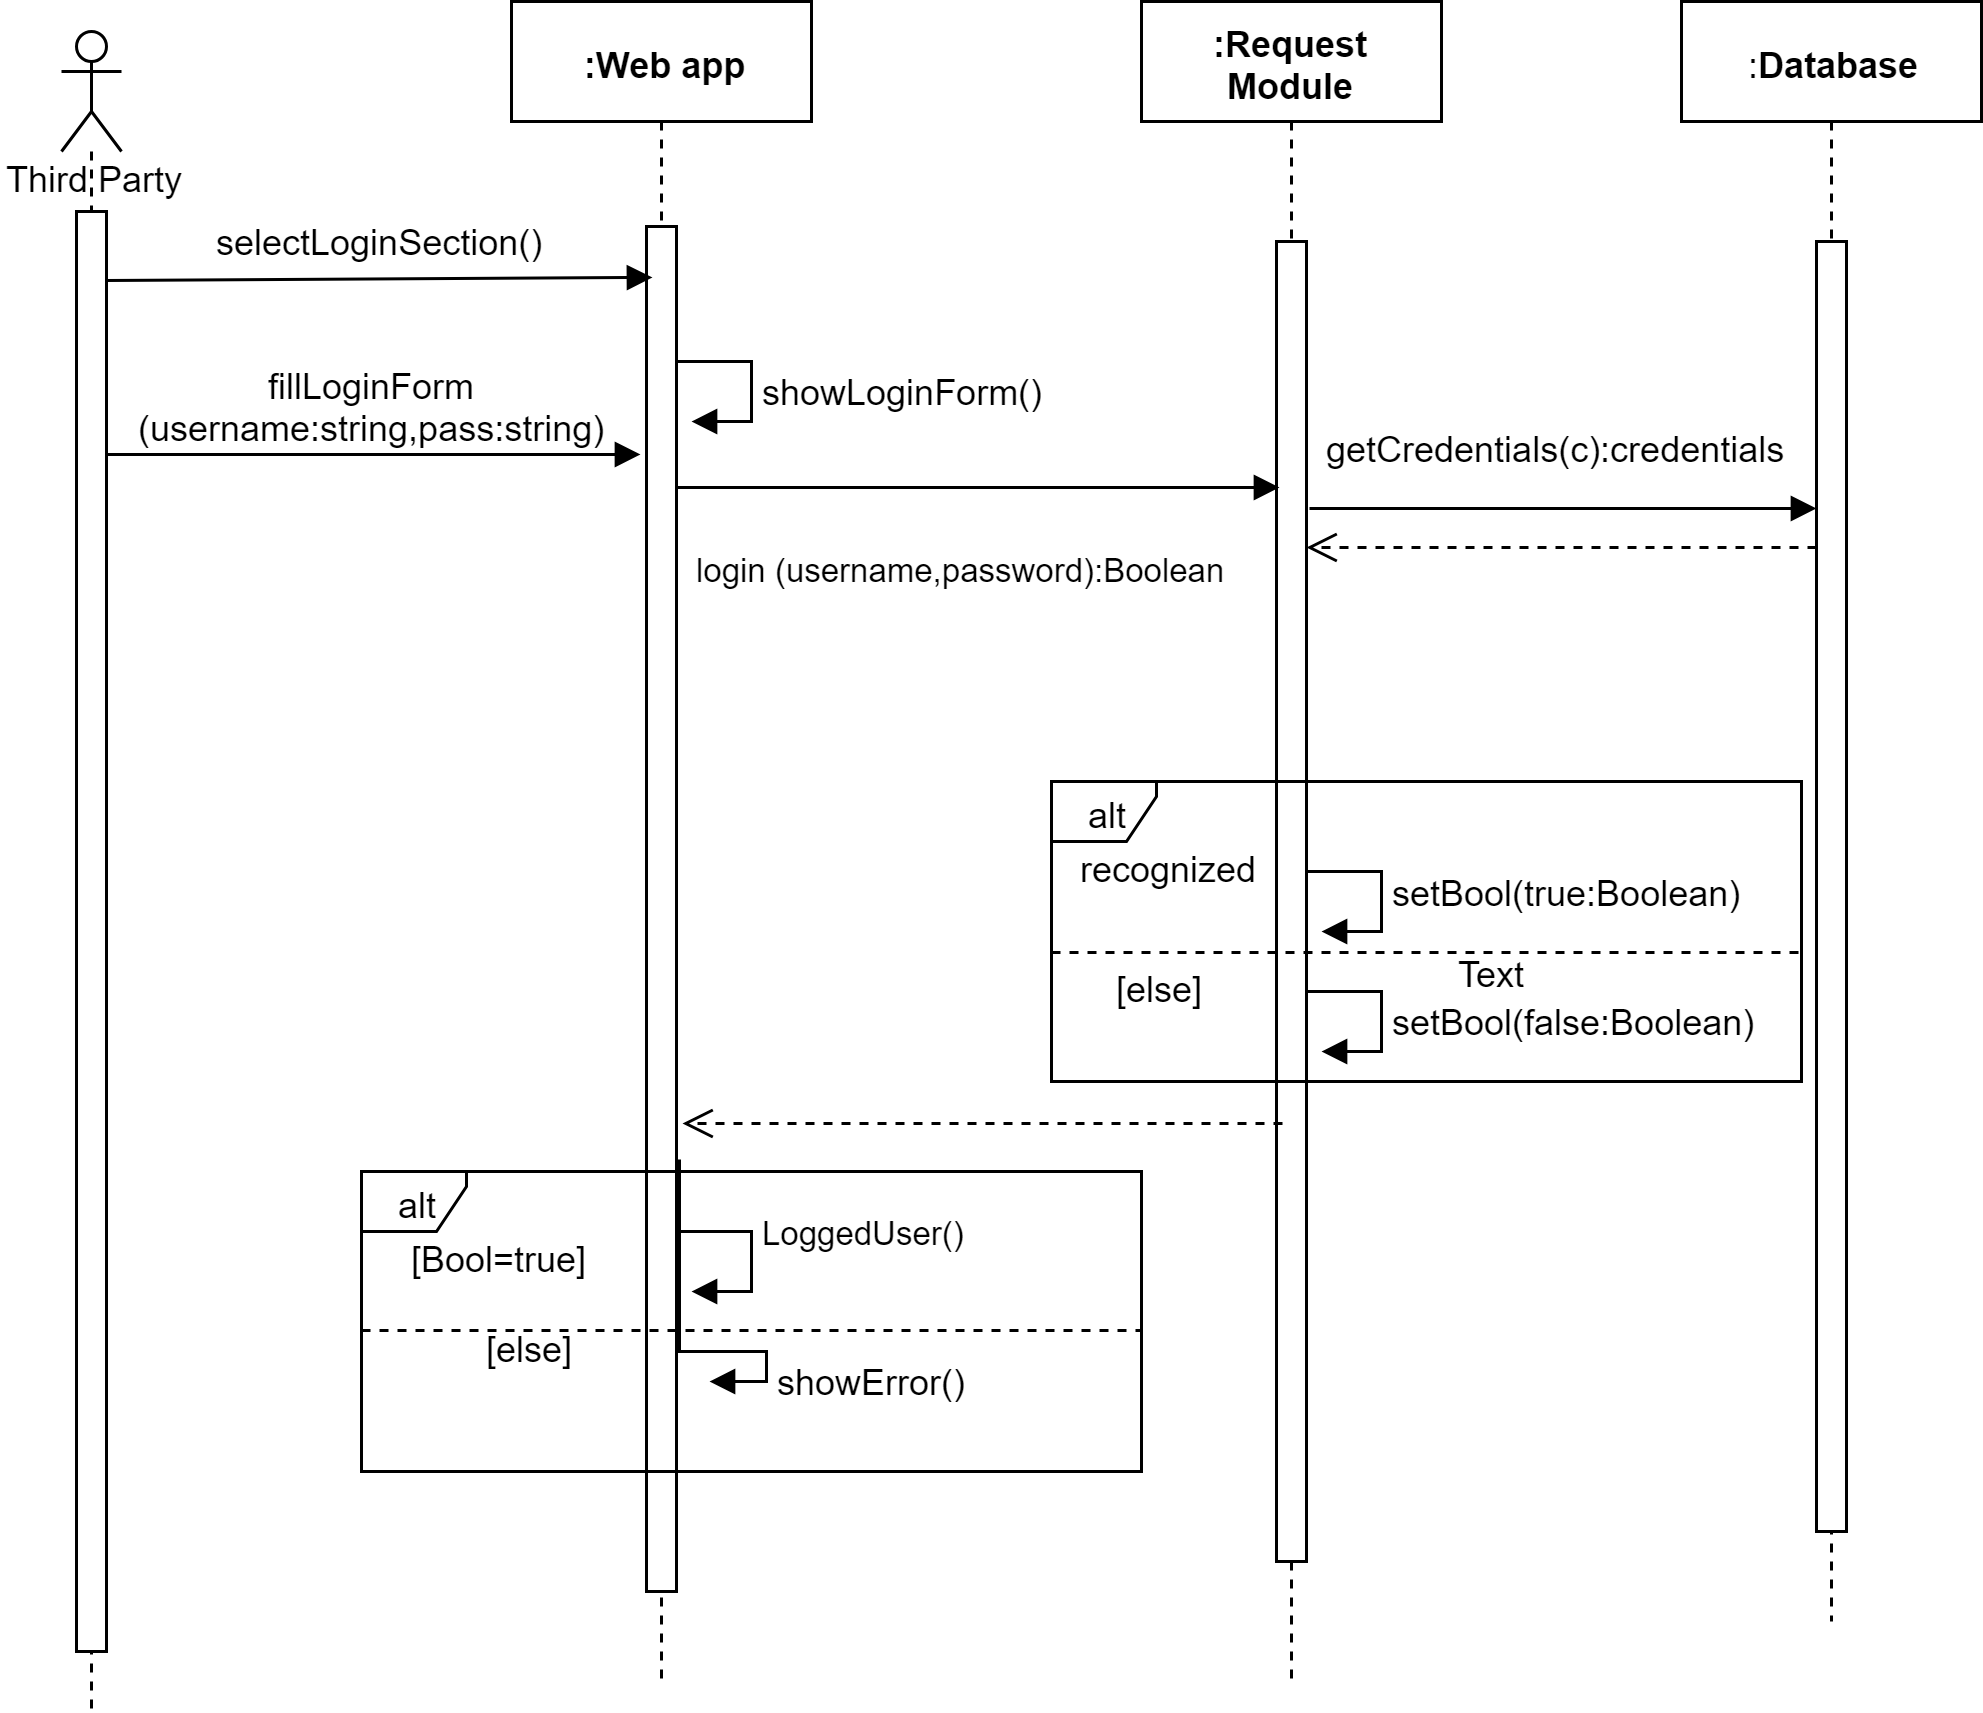
\includegraphics[scale=0.35]{./Pictures/login.png}
    \caption{Login sequence diagram}
\end{figure}

\begin{figure}[H]
    \centering
    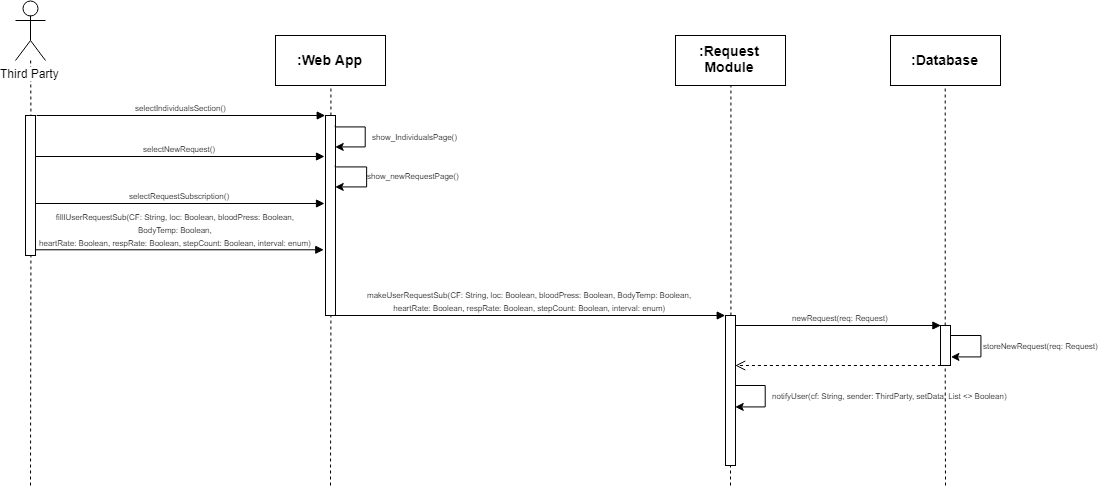
\includegraphics[scale=0.35]{./Pictures/userRequest.png}
    \caption{User request by a Third Party}
\end{figure}

\begin{figure}[H]
    \centering
    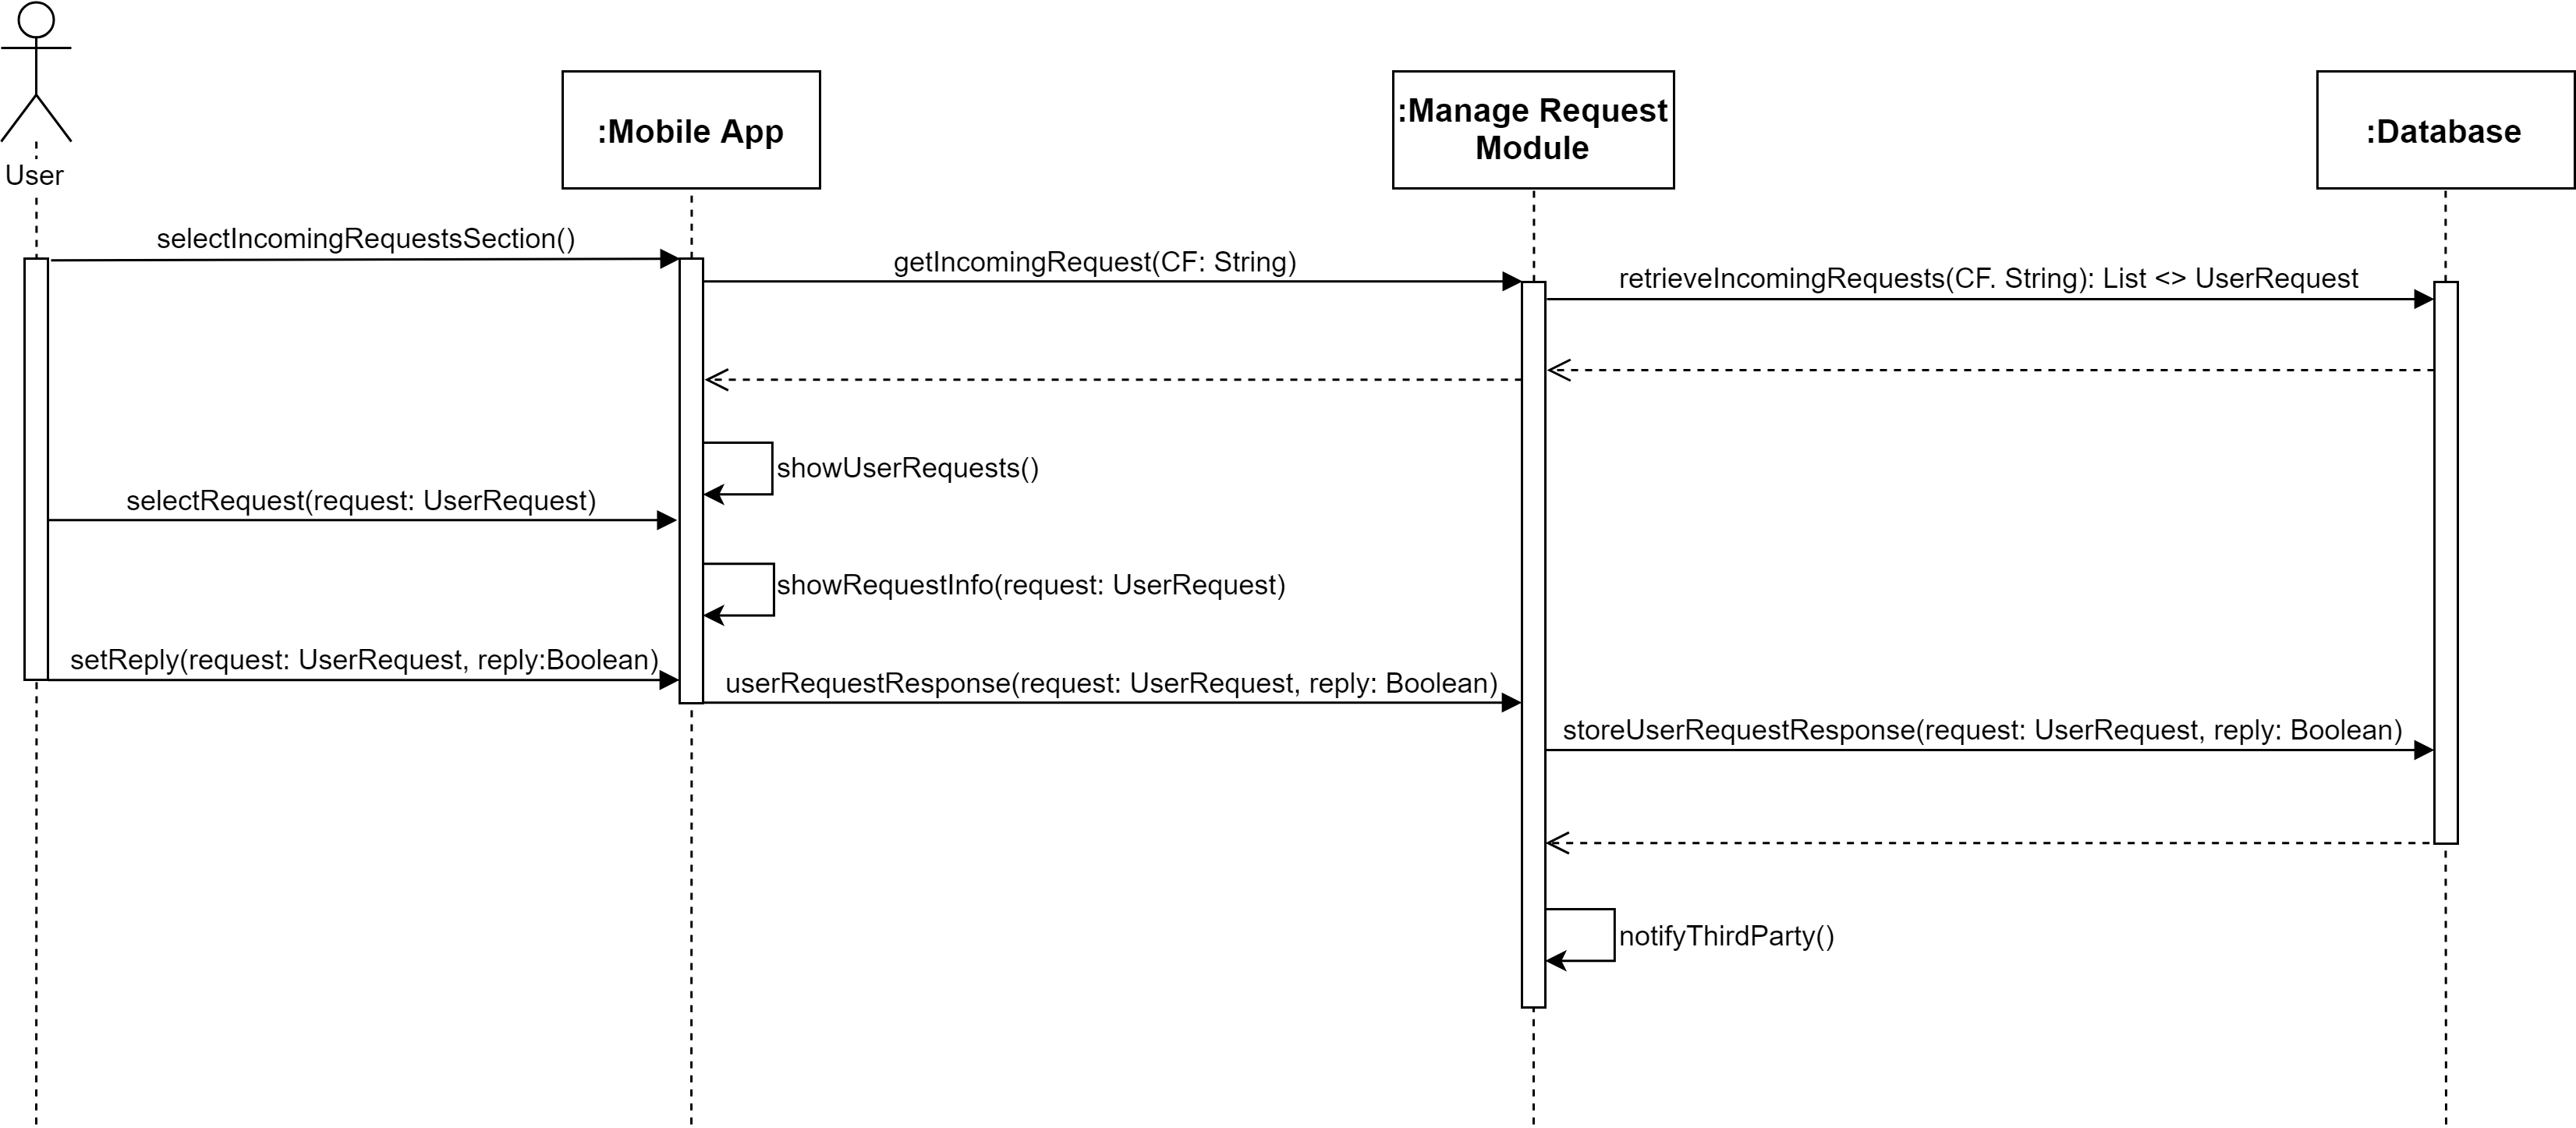
\includegraphics[scale=0.35]{./Pictures/acceptRequest.png}
    \caption{User acceptance of a request made by a Third Party}
\end{figure}

\begin{figure}[H]
    \centering
    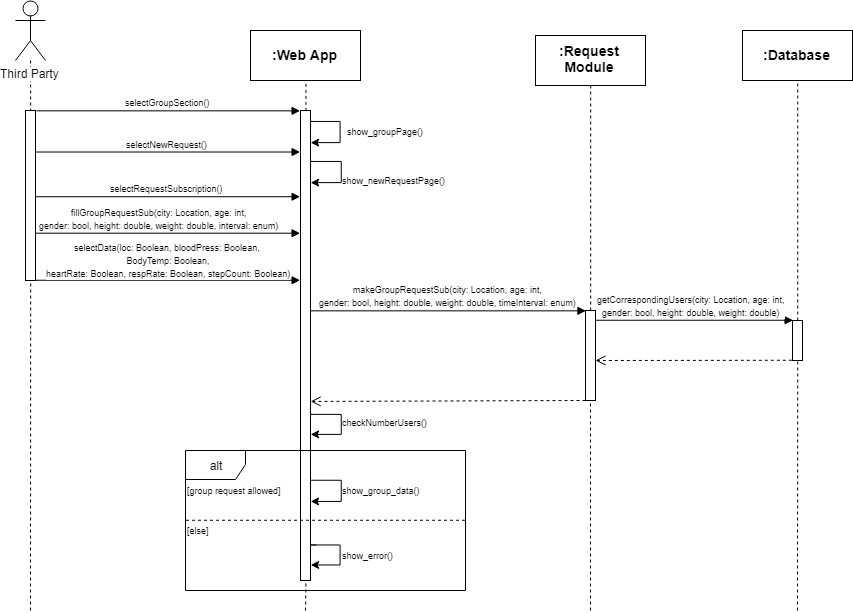
\includegraphics[scale=0.35]{./Pictures/groupRequestSeqDiagDD.png}
    \caption{Group request by a Third Party}
\end{figure}

\begin{figure}[H]
    \centering
    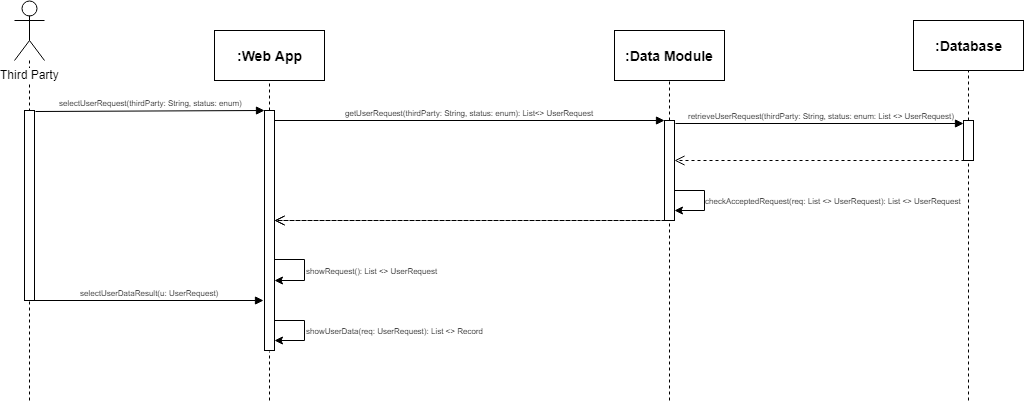
\includegraphics[scale=0.35]{./Pictures/showDataResult.png}
    \caption{Visualization of data of an already accepted request}
\end{figure}

%emergency sequence diagram

\begin{figure}[H]
    \centering
    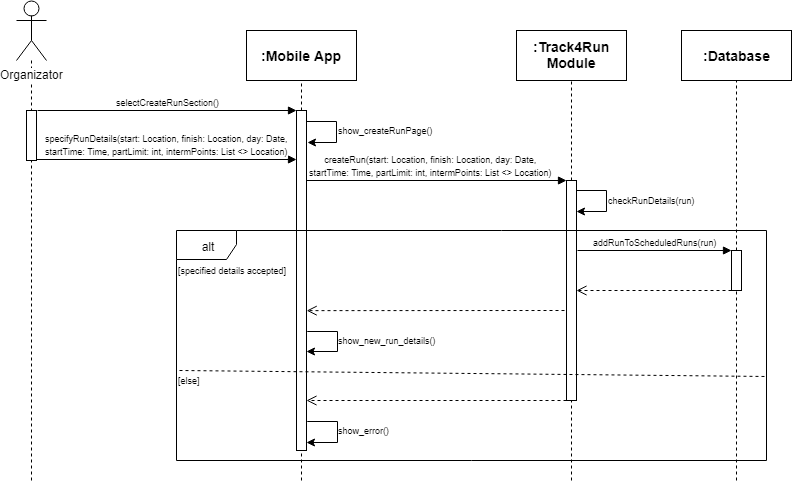
\includegraphics[scale=0.35]{./Pictures/createRunSeqDiagDD.png}
    \caption{Create a new run by an Organizator}
\end{figure}

\begin{figure}[H]
    \centering
    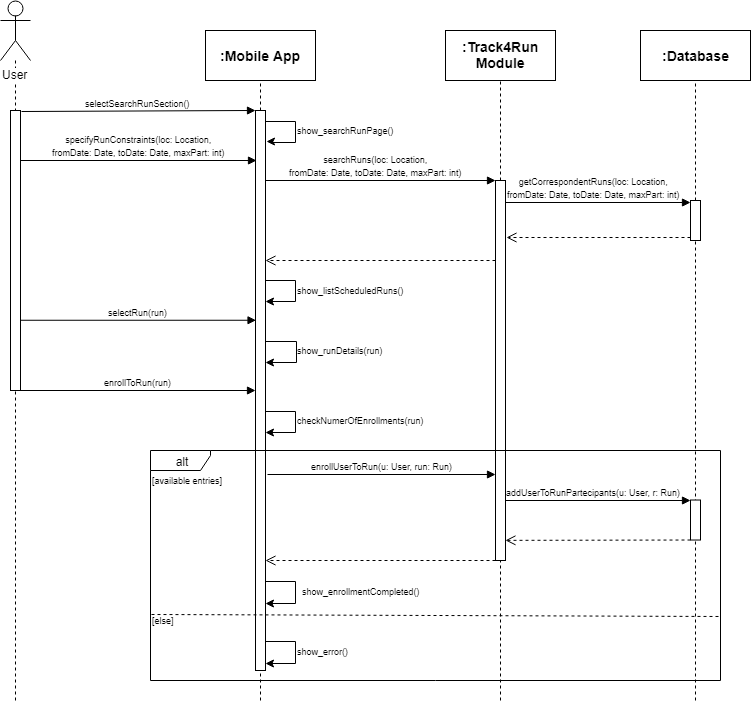
\includegraphics[scale=0.35]{./Pictures/enrollSeqDiagDD.png}
    \caption{Enrollment to a scheduled run by a User}
\end{figure}